% TU Delft beamer template
% Author: Erwin Walraven (initial version was created by Maarten Abbink)
% Delft Universiy of Technology

\documentclass{beamer}
\usepackage{amsmath}
\usepackage{amsfonts}
\usepackage{amsthm}
\usepackage{mathtools}
\usepackage[english]{babel}
\usepackage{calc}
\usepackage[absolute,overlay]{textpos}
\usepackage{graphicx}
\usepackage{subfig}
\usepackage{comment}
%\usepackage{tikz}
\usepackage{wasysym}
\usepackage{gensymb}
\usepackage{amssymb}
\usepackage{nccmath}
\usepackage{empheq}
\usepackage{xcolor}
\usepackage{relsize}
%\usepackage{apalike}
\usepackage[utf8]{inputenc}
\usepackage{multimedia}
\usepackage{media9}
%\usepackage{hyperref}.


\usepackage{arydshln}


\makeatletter
\renewcommand*\env@matrix[1][*\c@MaxMatrixCols c]{%
	\hskip -\arraycolsep
	\let\@ifnextchar\new@ifnextchar
	\array{#1}}
\makeatother


\newcommand*\widefbox[1]{\fbox{\hspace{1em}#1\hspace{1em}}}
%\useoutertheme{miniframes}

%\usefonttheme[onlymath]{serif}



\setbeamertemplate{navigation symbols}{} % remove navigation symbols
\mode<presentation>{\usetheme{tud}}


%\ExecuteBibliographyOptions{parentracker=false}



% BIB SETTINGS
%\usepackage[backend=bibtex,firstinits=true,maxnames=30,maxcitenames=20,url=false,style=authoryear]{biblatex}
%\bibliography{MyBib}
%\addbibresource{MyBib.bib}
%\setlength\bibitemsep{0.3cm} % space between entries in the reference list
%\renewcommand{\bibfont}{\normalfont\scriptsize}
%\setbeamerfont{footnote}{size=\tiny}
%\makeatletter
%\renewcommand{\cite}[1]{\footnote<.->[frame][{\fullcite{#1}}]}
%\renewcommand{\cite}[1]{$[$\cite{#1}$]$}


% Insert frame before each subsection (requires 2 latex runs)
\AtBeginSection {
	\begin{frame}<beamer>[noframenumbering] \frametitle{\titleSubsec}
		\tableofcontents[currentsection,currentsubsection]  % Generation of the Table of Contents
	\end{frame}
}

% Define the title of each inserted pre-subsection frame
\newcommand*\titleSubsec{Outline}
% Define the title of the "Table of Contents" frame
\newcommand*\titleTOC{Outline}

\graphicspath{ {./images/} } 

\title[DLS Lab Seminar]{DLS Lab Seminar \vspace{15pt}}
\institute[]{Istituto Italiano di Tecnologia, Genova, Italy \vspace{20pt}}
\author{Octavio A. Villarreal Maga\~na \vspace{20pt}} %\scriptsize Committee:  \\ Prof.Dr.Ir. Nathan van de Wouw (TUDelft, supervisor) \\ \vspace{1.5pt} \hspace{-11pt}Prof.Dr.Ir. Emmanuel Detournay (UMN, supervisor) \\ \vspace{-2.5pt} \hspace{-74pt}Dr.Ir. Manuel Mazo Jr. (TUDelft)}
\date{March 16th, 2017}

\begin{document}
{
\setbeamertemplate{footline}{\usebeamertemplate*{minimal footline}}
\frame{\titlepage}
\begin{frame}\frametitle{\titleTOC}
	\tableofcontents
\end{frame}
}

{\setbeamertemplate{footline}{\usebeamertemplate*{minimal footline}}
}

\section{Control structure}

\begin{frame}{Motivation}
	\begin{itemize}\setlength\itemsep{3em}
		\item Provide versatility to the types of gaits that the robot can perform
		\item Have a unified and systematic way to generate motions of the legs according to the scenario
		\item Can be applied to other legged systems
	\end{itemize}
\end{frame}

\begin{frame}{General picture}	
	\begin{itemize}[notitemsep, topsep=0pt]
		\item <1|only@1> [] 
		\begin{figure}[ht]\centering
			\hspace{-25pt}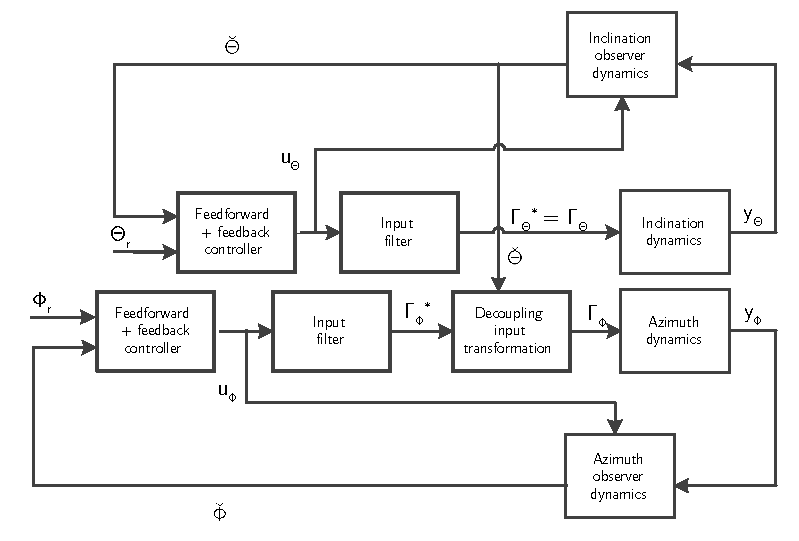
\includegraphics[width=1\textwidth]{images/ControlStrategy.pdf}
		\end{figure}
		\item <2|only@2> [] 
		\begin{figure}[ht]\centering
			\hspace{-25pt}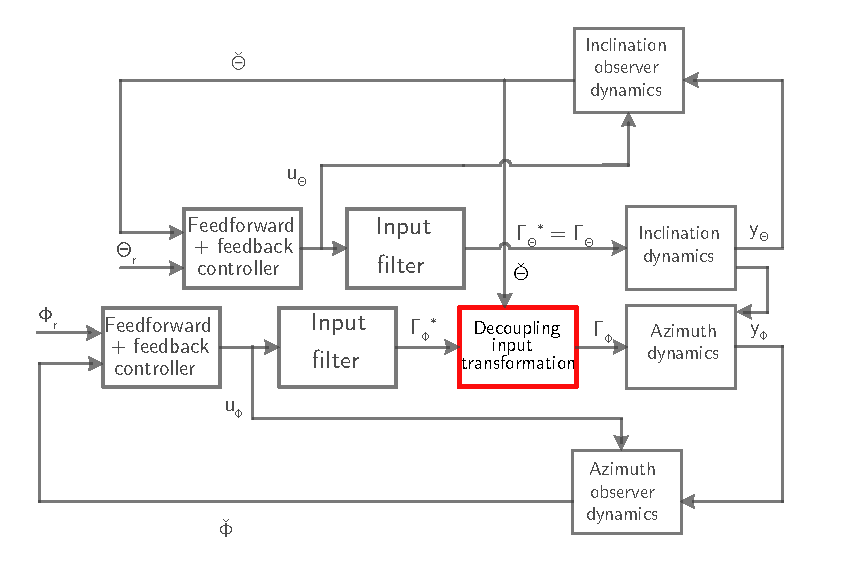
\includegraphics[width=1\textwidth]{images/ControlStrategy1.pdf}
		\end{figure}
	\end{itemize}
\end{frame}

\begin{frame}\frametitle{Supervisory controller}
	\begin{block}{Main goal}
		\Large Provide \textbf{geometrical} and \textbf{time} gait parameters, based on sensory data, to overcome the scenario that the robot is facing.
	\end{block}
\end{frame}



\begin{frame}{Supervisory controller (continue)}
		\begin{columns}
		\hspace{1cm}
		\begin{column}{0.5\textwidth}
		Geometrical parameters:
		\begin{itemize}
			\setlength\itemsep{3em}
			\item Step height $H_s$
			\item Step length $L_s$
			\item Oscillator "primitive" shape changes
		\end{itemize}	
		
		\end{column}
		\begin{column}{0.5\textwidth}
			\begin{figure}[ht]\centering
				\includegraphics[width=0.75\textwidth]{images/Supervisory.pdf}
			\end{figure}
			\begin{figure}[ht]\centering
				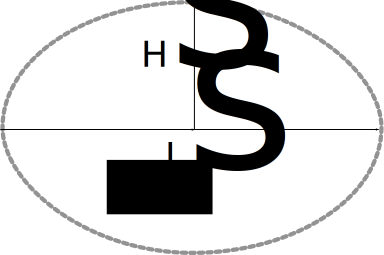
\includegraphics[width=0.75\textwidth]{images/PrimitiveShape.pdf}
			\end{figure}	
		\end{column}
		\end{columns}
\end{frame}

\begin{frame}{Supervisory controller (continue)}
		\begin{columns}
		\hspace{1cm}
		\begin{column}{0.5\textwidth}
		Time parameters:
		\begin{itemize}
			\setlength\itemsep{3em}
			\item Duty factor $D_f$
			\item Step frequency $S_f$
			\item Gait parameterization $G$ (e.g., $G_{trot}=\{1,4\}\prec\{2,3\}$)
			\item Time difference vector $\Delta$
		\end{itemize}	
		
		\end{column}
		\begin{column}{0.5\textwidth}
			\begin{figure}[ht]\centering
				\includegraphics[width=0.6\textwidth]{images/Supervisoryb.pdf}
			\end{figure}
			\vspace{-0.25cm}\begin{figure}[ht]\centering
							\includegraphics[width=0.22\textwidth]{images/Numbers.pdf}
			\end{figure}
			\begin{figure}[ht]\centering
				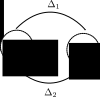
\includegraphics[width=0.45\textwidth]{images/TrotTime.pdf}
			\end{figure}
		\end{column}
		\end{columns}
\end{frame}

\begin{frame}{Max-plus gait scheduler}
	\begin{block}{Main goal}
		\Large Using the \textbf{time}-related gait parameters provided by the supervisory controller, generate the list of time-instants when each leg has to leave and touch the ground, so that a desired coordination is achieved.
	\end{block}
\end{frame}

\begin{frame}{Max-plus gait scheduler (continue)}
\begin{columns}
\hspace{1cm}
\begin{column}{0.45\textwidth}
	\begin{figure}[ht]\centering
		\includegraphics[width=0.9\textwidth]{images/MaxPlus.pdf}
	\end{figure}
	\begin{figure}[ht]\centering
		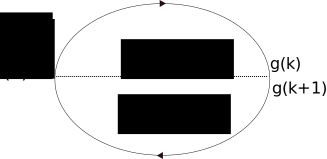
\includegraphics[width=0.9\textwidth]{images/Phases.pdf}
	\end{figure}
\end{column}
\begin{column}{0.55\textwidth}
$G_{trot}=\{1,4\}\prec\{2,3\}$ \\
$D_f = 0.58$ \\
$S_f = 0.42$ \\
$\Delta = [0.2,0.2]$ 

\begin{table}[]
\centering
\label{my-label}
\resizebox{\textwidth}{!}{\begin{tabular}{|l|l|l|l|l|l|l|l|l|}
\hline
$k$ & $g_1(k)$ & $g_2(k)$ & $g_3(k)$ & $g_4(k)$ & $l_1(k)$ & $l_2(k)$ & $l_3(k)$ & $l_4(k)$ \\ \hline
0   & 0        & 0        & 0        & 0        & 0        & 0        & 0        & 0        \\ \hline
1   & 2.4      & 3.6      & 3.6      & 2.4,     & 1.4      & 2.6      & 2.6      & 1.4      \\ \hline
2   & 4.8      & 6        & 6        & 4.8      & 3.8      & 5        & 5        & 3.8      \\ \hline
3   & 7.2      & 8.4      & 8.4      & 7.2      & 6.2      & 7.4      & 7.4      & 6.2      \\ \hline
4   & 9.6      & 10.8     & 10.8     & 9.6      & 8.6      & 9.8      & 9.8      & 8.6      \\ \hline
5   & 12       & 13.2     & 13.2     & 12       & 11       & 12.2     & 12.2     & 11       \\ \hline
\end{tabular}}
\end{table}
\end{column}
\end{columns}
\end{frame}

\begin{frame}{Max-plus gait scheduler (continue)}
\begin{itemize}
	\setlength\itemsep{2em}
	\item Systematic gait generation 
	\item No coupling matrix $\mathbb{C}_{ij}$
	\item Total cycle time analysis (max-plus eigenvalues of $A$ matrix in $x(k+1) = A\otimes x(k)$)
	\item Coupling time analysis ("settling time")
	\item Not computationally expensive
	\item Possibility to provide "optimal" gait switching
\end{itemize}	
\end{frame}

\begin{frame}{Angular frequency reference generator}
	\begin{block}{Main goal}
		\Large Making use of the \textbf{touchdown} and \textbf{lift-off} times of the max-plus gait scheduler, provide a function for the evolution of the angular frequency of the oscillator-based reference generator.
	\end{block}
\end{frame}

\begin{frame}{Angular frequency reference generator (continue)}
\begin{columns}
\begin{column}{0.5\textwidth}
\begin{itemize}
	\item Stance and swing period:
	\begin{align*}
	Ti_{st} &= l_i(k+1) - g_i(k) \\
	Ti_{sw} &= g_i(k+1) - l_i(k+1),
	\end{align*}
	\item Average angular frequency:
	\begin{equation*}
	\bar{\omega} = \begin{cases}
	\frac{\pi}{Ti_{st}} \textbf{ for } t \in [g_i(k),l_i(k+1)] \\
	\frac{\pi}{Ti_{sw}} \textbf{ for } t \in (l_i(k+1),g_i(k+1)] 
	\end{cases}\label{eq:angularfreq}
	\end{equation*}
	\item Condition for the angular frequency function:
	\begin{equation*}
	\frac{1}{Ti_{p}}\int^{Ti_{p}} \omega dt = \bar{\omega} \textbf{ for } p = st,sw.\label{eq:angularfrequencycondition}
	\end{equation*} 
\end{itemize}
\end{column}
\hspace{1cm}

\begin{column}{0.5\textwidth}
\begin{figure}[H]
			\includegraphics[width=0.7\textwidth]{AngularFrequency.pdf}
\end{figure}
\begin{figure}[H]
			\includegraphics[width=0.8\textwidth]{PhasesPeriod.pdf}
\end{figure}
\end{column}
\end{columns}
\end{frame}

\begin{frame}{Angular frequency reference generator (continue)}
\centering$\omega = \bar{\omega}$
\begin{figure}[H]\centering
			\includegraphics[width=1\textwidth]{HeightTime.png}
\end{figure}
\end{frame}

\begin{frame}{Oscillator continuous time reference generator}
	\begin{block}{Main goal}
		\Large Generate reference trajectories for each of the legs of the robot in such a way that the desired gait is achieved, according to the angular frequency obtained from the angular frequency reference generator.
	\end{block}
\end{frame}

\begin{frame}{Oscillator continuous time reference generator \\(continue)}
Oscillator equations:
\begin{align*}
x = \alpha (1 - \frac{16x^4}{L_s^4} - \frac{z^4}{H_s^4})x + \frac{1.18\omega L_s}{2H_s^3}z^3 \\
z = \beta (1 - \frac{16x^4}{L_s^4} - \frac{z^4}{H_s^4})z - \frac{9.44\omega H_s}{L_s^3}x^3
\end{align*}
\begin{figure}[t]
		\centering
		\begin{minipage}[t]{0.4\textwidth}
			\centering
			\includegraphics[width=0.6\linewidth]{images/Oscillator.pdf}\\
		\end{minipage}%\\
		\begin{minipage}[t]{0.6\textwidth}
			\vspace{-2.5cm}
			\centering
			\includegraphics[width=1\linewidth]{images/LimitCycle.png}\\
		\end{minipage}
\end{figure}
\end{frame}




\section{Numeric simulations}


\begin{frame}{Parameters used}
Switch between four different sets of gait parameters:
\begin{table}[b]
\centering
\label{Table:GaitParameters}
\resizebox{\textwidth}{!}{\begin{tabular}{|l|l|l|l|l|}
\hline
       & $G$                                   & $D_f$ & $S_f[\frac{1}{s}]$ & $\Delta[s]$                                                 \\ \hline
$T_1$ & $\{1,4\}\prec\{2,3\}$                 & 0.6  & 1/3        & $[0.2, 0.4]$               \\ \hline
$T_2$ & $\{1,4\}\prec\{2,3\}$                 & 0.4  & 1/3        &$[-0.2,-0.4]$                \\ \hline
$W_1$ & $\{1\}\prec\{2\}\prec\{3\}\prec\{4\}$ & 0.6  & 1/3       & $[-0.45 , -0.45 , -0.45 , -0.45]$     \\ \hline
$W_2$ & $\{1\}\prec\{2\}\prec\{3\}\prec\{4\}$ & 0.4  & 1/3     & $[ -1.4 , -0.7 , -1.4 , -0.7]$ \\ \hline
\end{tabular}}
\end{table}
\end{frame}

\begin{frame}{Generated motion references}
\begin{figure}[H]\centering
	\includegraphics[width=1\textwidth]{SyncPlot.png}
\end{figure}
\end{frame}

\begin{frame}{Duty factor}
\vspace{-1cm}
	\begin{figure}[ht]\centering
		\includegraphics[width=1.1\textwidth]{images/DutyFactor.png}
	\end{figure}\vspace{-20pt}
\end{frame}

\begin{frame}{Animation}

\begin{center}
        \movie[width=\textwidth,showcontrols=true]
        {\includegraphics[width=\textwidth]{Legs.png}}{Legs.mp4} \\
\end{center}

\end{frame}

\section{Further work}


\begin{frame}{Further work}
	\begin{itemize}\setlength\itemsep{0.5em}
		\item Use the proposed strategy in the current framework
		\item Design angular frequency generator
		\item Account for disturbances in the max-plus algebra gait scheduler
		\item Design of supervisory parameters according to sensory information
		\item Design transition between one set of parameters to another
	\end{itemize}
\end{frame}

\begin{frame}
 \hspace{2cm} Thank you. Questions or comments?
\end{frame}





\end{document}
